\documentclass[aspectratio=169]{../latex_main/tntbeamer}  % you can pass all options of the beamer class, e.g., 'handout' or 'aspectratio=43'
\usepackage{dsfont}
\usepackage{bm}
\usepackage[english]{babel}
\usepackage[T1]{fontenc}
%\usepackage[utf8]{inputenc}
\usepackage{graphicx}
\graphicspath{ {./figures/} }
\usepackage{algorithm}
\usepackage[ruled,vlined,algo2e,linesnumbered]{algorithm2e}
\usepackage{hyperref}
\usepackage{booktabs}
\usepackage{mathtools}

\usepackage{amsmath,amssymb}

\DeclareMathOperator*{\argmax}{arg\,max}
\DeclareMathOperator*{\argmin}{arg\,min}

\usepackage{pgfplots}
\pgfplotsset{compat=1.16}
\usepackage{tikz}
\usetikzlibrary{trees} 
\usetikzlibrary{shapes.geometric}
\usetikzlibrary{positioning,shapes,shadows,arrows,calc,mindmap}
\usetikzlibrary{positioning,fadings,through}
\usetikzlibrary{decorations.pathreplacing}
\usetikzlibrary{intersections}
\pgfdeclarelayer{background}
\pgfdeclarelayer{foreground}
\pgfsetlayers{background,main,foreground}
\tikzstyle{activity}=[rectangle, draw=black, rounded corners, text centered, text width=8em]
\tikzstyle{data}=[rectangle, draw=black, text centered, text width=8em]
\tikzstyle{myarrow}=[->, thick, draw=black]

% Define the layers to draw the diagram
\pgfdeclarelayer{background}
\pgfdeclarelayer{foreground}
\pgfsetlayers{background,main,foreground}

% Requires XeLaTeX or LuaLaTeX
\usepackage{unicode-math}

\usepackage{fontspec}
%\setsansfont{Arial}
\setsansfont{RotisSansSerifStd}[ 
Path=../latex_main/fonts/,
Extension = .otf,
UprightFont = *-Regular,  % or *-Light
BoldFont = *-ExtraBold,  % or *-Bold
ItalicFont = *-Italic
]
\setmonofont{Cascadia Mono}[
Scale=0.8
]

% scale factor adapted; mathrm font added (Benjamin Spitschan @TNT, 2021-06-01)
%\setmathfont[Scale=1.05]{Libertinus Math}
%\setmathrm[Scale=1.05]{Libertinus Math}

% other available math fonts are (not exhaustive)
% Latin Modern Math
% XITS Math
% Libertinus Math
% Asana Math
% Fira Math
% TeX Gyre Pagella Math
% TeX Gyre Bonum Math
% TeX Gyre Schola Math
% TeX Gyre Termes Math

% Literature References
\newcommand{\lit}[2]{\href{#2}{\footnotesize\color{black!60}[#1]}}

%%% Beamer Customization
%----------------------------------------------------------------------
% (Don't) Show sections in frame header. Options: 'sections', 'sections light', empty
\setbeamertemplate{headline}{empty}

% Add header logo for normal frames
\setheaderimage{
	% 
\includegraphics[height=\logoheight]{figures/TNT_darkv4.pdf}
	
\includegraphics[height=\logoheight]{../latex_main/figures/luh_logo_rgb_0_80_155.pdf}
	% 
\includegraphics[height=\logoheight]{figures/logo_tntluh.pdf}
}

% Header logo for title page
\settitleheaderimage{
	% 
\includegraphics[height=\logoheight]{figures/TNT_darkv4.pdf}
	
\includegraphics[height=\logoheight]{../latex_main/figures/luh_logo_rgb_0_80_155.pdf}
	% 
\includegraphics[height=\logoheight]{figures/logo_tntluh.pdf}
}

% Title page: tntdefault 
\setbeamertemplate{title page}[tntdefault]  % or luhstyle
% Add optional title image here
%\addtitlepageimagedefault{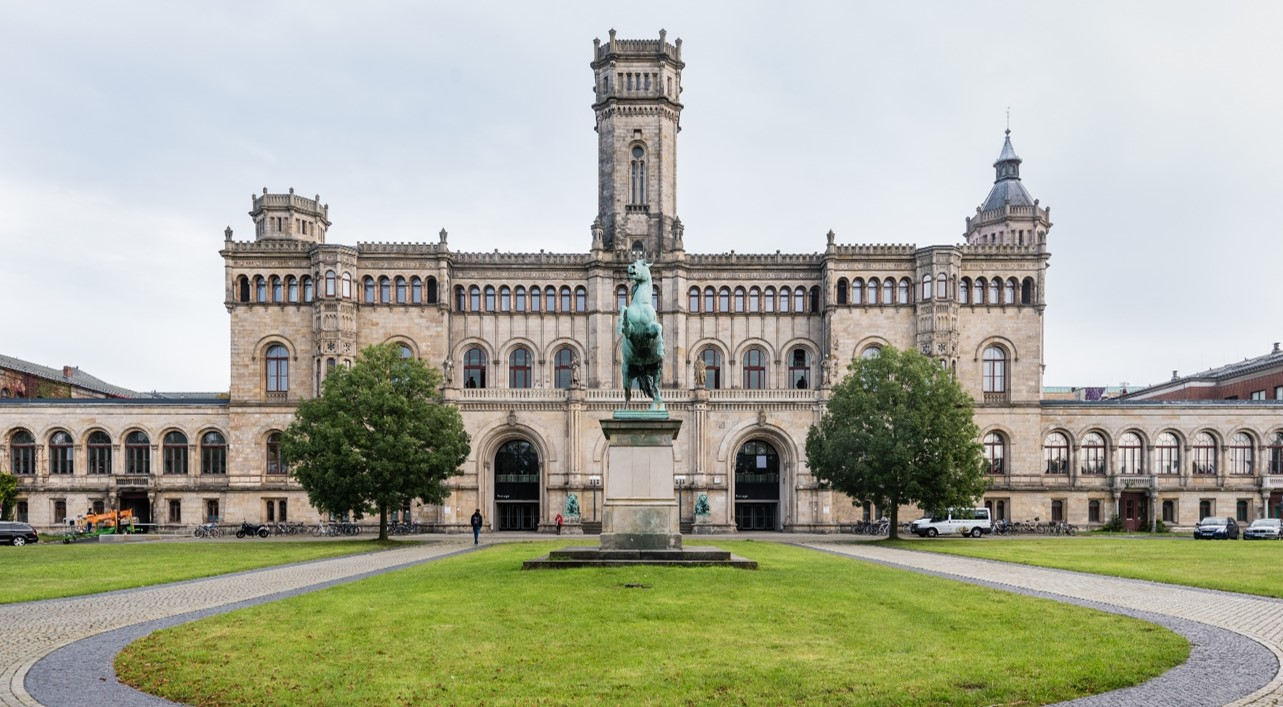
\includegraphics[width=0.65\textwidth]{figures/luh_default_presentation_title_image.jpg}}

% Title page: luhstyle
% \setbeamertemplate{title page}[luhstyle]
% % Add optional title image here
% \addtitlepageimage{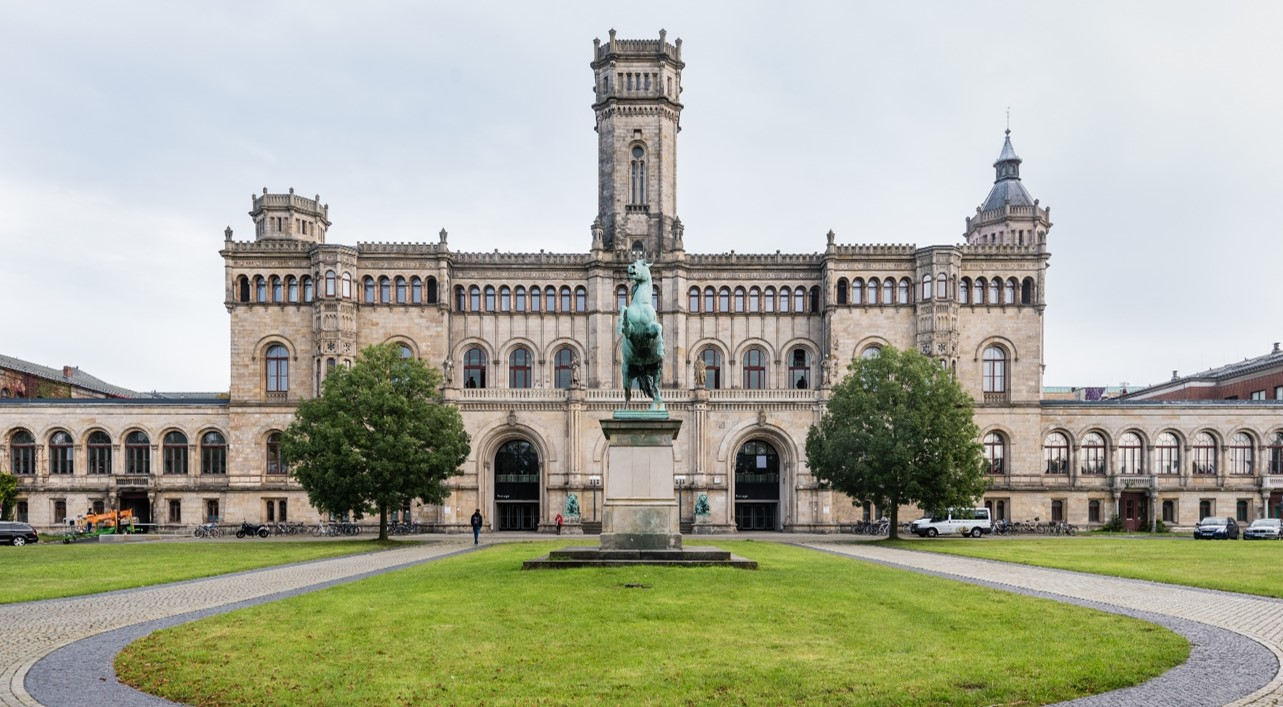
\includegraphics[width=0.75\textwidth]{figures/luh_default_presentation_title_image.jpg}}

\author[Lindauer \& Anand]{Marius Lindauer and Avishek Anand\\[1em]
	
\includegraphics[height=\logoheight]{../latex_main/figures/luh_logo_rgb_0_80_155.pdf}\qquad

\includegraphics[height=\logoheight]{../latex_main/figures/TNT_darkv4}\qquad

\includegraphics[height=\logoheight]{../latex_main/figures/L3S.jpg}	}
\date{Winter Term 2021
}


%%% Custom Packages
%----------------------------------------------------------------------
% Create dummy content
\usepackage{blindtext}

% Adds a frame with the current page layout. Just call \layout inside of a frame.
\usepackage{layout}


\title[Introduction]{iML: Introduction}
\subtitle{Properties}
%\institute{}

\begin{document}
	
	\maketitle


\begin{frame}[c]{How to Measure Interpretability?}
	
	\begin{itemize}
	    \item No real metric, but only proxies such as complexity of the model or the explanation
	    \pause
	    \item \lit{Doshi-Velez and Kim 2017}{https://arxiv.org/abs/1702.08608} proposed three main levels of interpretability
	    \begin{description}
	        \item[Real Task] Apply in production and study whether users are satisfied
	        \begin{itemize}
	            \item[$\leadsto$] Crazy expensive, but actually what you want
	        \end{itemize}
	        \pause
	        \item[Simple Task] Apply it to a simplified application and evaluate it by laypersons
	        \begin{itemize}
	            \item[$\leadsto$] fairly expensive, but only approximation of the real world
	        \end{itemize}
	        \pause
	        \item[Proxy Task] instead of real tasks; e.g., tree depth for a measure of complexity
	        \begin{itemize}
	            \item[$\leadsto$] cheap, but often only crude approximation of real interpretability
	        \end{itemize}
	        
	    \end{description}
	\end{itemize}
	
\end{frame}



\begin{frame}[c]{Properties of Explanation Methods \lit{Robnik-Sikonja and Bohanec 2018}{https://link.springer.com/chapter/10.1007/978-3-319-90403-0_9}}
	
	\begin{description}
        \item[Expressive Power] is the power of which kind of models (e.g., decision boundaries) can be expressed 
        \begin{itemize}
            \item More expressive power is nice for accuracy, but can hurt interpretability
        \end{itemize}
        \medskip
        \pause
        \item[Translucency] measures how much information of the model is used
        \begin{itemize}
            \item black-box approaches only observing input and output of models\\ are not translucent
            \item using the model weights (e.g., of linear regression) would be high translucent
        \end{itemize}
        \medskip
        \pause
        \item[Portability] describes to how many model classes method can be applied to
        \begin{itemize}
            \item not translucent model are often very portable
        \end{itemize}
        \medskip
        \pause
        \item[Algorithmic Complexity] describes how much compute resources are needed to\\ compute the explanation
        \begin{itemize}
            \item should be scale well with number of observations and features if possible
        \end{itemize}
        
	\end{description}
\end{frame}

\begin{frame}[c]{Properties of Individual Explanations~\lit{Robnik-Sikonja and Bohanec 2018}{https://link.springer.com/chapter/10.1007/978-3-319-90403-0_9}}
	
	\begin{description}
        \item[Accuracy] How accurate is the explanation on unseen data? Similar to accuracy of models.
        \begin{itemize}
            \item If this is too small, there might be no point in using it\\ since it does not reflect the ``real world''.
        \end{itemize}
        \medskip
        \pause
        \item[Fidelity] How accurately does the explanation reflect the predictions of the model? 
        \begin{itemize}
            \item If this is too small, there is no point in using it\\ since it does not reflect the model to be explained.
        \end{itemize}
        \medskip
        \pause
        \item[Consistency] measures how much explanation of two models trained on the same task differ. 
        \begin{itemize}
            \item Desirable if both models rely on the same features and relationships
        \end{itemize}
        \medskip
        \pause
        \item[Comprehensibility] Can the human comprehend the model?
        \begin{itemize}
            \item hard to measure (see before)
        \end{itemize}
	\end{description}
\end{frame}

\begin{frame}[c]{Properties of Individual Explanations (cont'd)~\lit{Robnik-Sikonja and Bohanec 2018}{https://link.springer.com/chapter/10.1007/978-3-319-90403-0_9}}
	
	\begin{description}
        \item[Certainty] Does the explanation reflect the certainty of the model?
        \begin{itemize}
            \item Important for probabilistic models with uncertainty estimates
            \item Explanation should not be more uncertain or certain than the original model
        \end{itemize}
        \medskip
        \pause
        \item[Degree of Importance] Can the explanation explain the importance of features and interaction effects?
        \begin{itemize}
            \item Often interesting for users to know which feature was most important
        \end{itemize}
        \medskip
        \pause
        \item[Novelty] Can the explanation also reflect that a new observation is far from the original data distribution used for training?
        \begin{itemize}
            \item Should ideally also lead to high uncertainty in the explanation (and model)
        \end{itemize}
        \pause
        \item[Representativeness] Does the explanation cover only a single (or few) observations or all of them?
        \begin{itemize}
            \item Whether more or less is better depends on the application
        \end{itemize}
        
	\end{description}
\end{frame}
	
\end{document}
